%\chapter{Creating the Biomedical Question Answering System}

%
\section{Team coding with GitHub}

You will again use GitHub to host your project code. But different from previous
homeworks, all the team members need to collaborate on the project, and commit
the code changes to the same repository, which means it is good to learn how to
more about git and GitHub in this subtask.

\subsection{Creating a repository}

\begin{enumerate}

\item The team leader needs to create a repository with his/her GitHub acccount,
and name your project as \texttt{COURSENUM-teamID}, where \texttt{ID} is your team
number, which is a two-digit number ranging from 01 to 18. If you are not sure
how to create a GitHub repository, please refer to Homework 0.

At this point, all the team members are able to checkout the empty project and
start working on their own. But this is NOT recommended! We recommend the team
leader could checkout the project from GitHub repository, go through the entire
Maven project building process (we will come to this in the next subtask) until
you can run a simple pipeline. Then, the team leader again, from
his/her laptop, commits and pushes everything to the repository before the team
members clone the project.

\item Now, everyone has the read permission to your project repository (since it
is a public repository). To help your team members gain read/write permissions,
you, the team leader, should add them as collaborators. You need to click the
\textbf{Admin} tab on your project homepage, and click the
\textbf{Collaborators} menu on the left. Put in your teammates' GitHub IDs one
by one, and click \textbf{Add} button.

\end{enumerate}

\subsection{Creating milestones, issues, and Wiki pages}

To create milestones for your development will help better organize your team
members, know your collaborators' progress, and help users/customers know what
they could expect from a future release. Issues can be detailed action items
team members would like to contribute to each milestone. Action can be bug fix,
feature enhancement, etc. If you are still unclear what a milestone is or what
an issue is, or you want to understand how milestone and issue tracking system
can help software development, we recommended that you read about the features of GitHub
issue tracking system at
\url{https://github.com/blog/831-issues-2-0-the-next-generation} and
\url{https://github.com/features/projects/issues}.

We recommend all the team members have a discussion on how to set the
milestones, and what your first several initial issues will be (i.e., what they
first couple of things you want to do at the beginning.) And the team leader
does the following steps. \textbf{Remember that you are unlikely to submit all
the issues to the tracking system at once, you may create new issues for bugs to
fix or new features to implement, change the owner (assignee) of the issue,
close implemented issues, or mark some as wontfix. All your team members
are responsible to maintain your milestones and issues.}

\begin{enumerate}

\item To create a milestone, you can navigate to the \textbf{Issues} tab of your
project homepage, then click the \textbf{Milestones} below the main menu bar.
Now you are able to see the button \textbf{Create a new milestone}, and click it.

\item Type your title for the milestone, e.g., ``M1'' for the first milestone
(you can also make it more meaningful and specific). Write a few descriptions
for this milestone, like the goal and the brief descriptions of features will be
enhanced in this milestone. Finally, select a ``Due Data'' for the milestone.
Click the ``Create Milestone'' to finalize creating your milestone.

\item Do the previous step once again until all your milestones are created.

\item Now, you need to submit your first several issues. Go back to the
\textbf{Issues} tab on your project homepage, and click \textbf{New Issue}. Type
a title, assign the task to a particular team member, link this issue to a
previously created milestone. Finally write down detailed comments to the issue.

You may find when you type ``@'' followed by your collaborator's ID in the
comment box, you are able to mention your collaborator as you mention your
friend in a tweet on Twitter.

You can learn how to write in GitHub Flavored Markdown language, by clicking the
link above the textbox.

You can also attch labels to each issue by selecting them from the right panel.
As we mentioned earlier, you can change the milestone assignment, in particular,
if you find you couldn't finish it by M1, then you can change it to M2 later, or
you can also relabel it as \textbf{wontfix}.

\end{enumerate}

Now, you can create a Wiki page for your team meeting minutes and other
important items.

\begin{enumerate}

\item Click the ``Wiki'' tab at the top of your project homepage, and click
\textbf{Edit Page} to start editing it.

\end{enumerate}

Once you reach this point, remember to send us an email to report the URL of
your project repository page (e.g., \url{https://github.com/COURSENUM-ID/project-teamID}).

\subsection{Team coding with git-branch, git-merge, git-rebase}

Collaboration is important for this homework. All the team members start their
individual development after the team leader gets the framework ready, and
pushes all his/her local commits to the repository. Once a team member finalizes
his/her development, he/she might take responsibility on another task, or want
to check the integrity or compatibility with features implemented by
collaborators. After all the individual developments are done, team leader is
responsible to merge all the newly developed components into the same codebase
and test the integrity.

Git branching is a good tool to help the team manage parallel development and
distributed codebase. In fact, the branching mechanism is widely adopted by not
only git, but many other version control systems, e.g., SVN or Mercurial (Hg).
But one of the most important reasons that people love git branching over SVN or
Mercurial (Hg) is its light-weight nature, which allow switching between
development branches within the same clone of a repository.

Normally, the team leader is in charge of the \texttt{master} branch (the one
you probably used for homework 0 and 1), which usually corresponds to a codebase
for the most recent stable release, while team members should create branches
for each individual task assignment, e.g., bug fixes, feature enhancement with
\texttt{git branch} command. You can also do it within Eclipse by right-clicking
the project name, and select \textbf{Team} $\rightarrow$ \textbf{Switch To}
$\rightarrow$ \textbf{New Branch\ldots}.

To merge multiple development branches back to \texttt{master} branch (or in
Eclipse \textbf{Team} $\rightarrow$ \textbf{Switch To} $\rightarrow$
\textbf{master}), you should switch back to master, and then \texttt{git merge}
the branch you want to be merged (or \textbf{Team} $\rightarrow$
\textbf{Merge\ldots}). Sometimes, you may also need \texttt{git rebase} when you
later realize your development should depend on another feature that was also
being developed by your collaborator, which hadn't beed integrated in the
\texttt{master} branch by the time you created your development branch.

To better understand git branching, you should read the ``Git Branching''
chapter of Pro Git Book (\url{http://git-scm.com/book/en/Git-Branching}). You
can also find a more sophisticated branching model at
\url{http://nvie.com/posts/a-successful-git-branching-model/}, which may be too
complicated for this homework, but it can inspire how you want to manage your
branches.

If you are looking for a Eclipse plug-in that can bring the GitHub issue
tracking system to your workspace, e.g., create/close/comment issues, label
them, assign to a person within eclipse, or automatically get notified by a
message bubble if an issue is assigned to you, then you can try to investigate
Mylyn plug-in. In the ``Tips and Tricks using Eclipse with Github''
post\footnote{
\url{http://eclipsesource.com/blogs/2012/08/28/tips-and-tricks-using-eclipse-with-github/}}
, you will find the basic idea how Mylyn GitHub connector works. By default,
Eclipse Juno for Java developers comes with EGit, Mylyn, and Mylyn Github
connector, and the Task View is on the top-right corner of the Java perspective
by default.

\chapter{Creating your first BioASQ pipeline}
\vspace{-1cm}
In this task you will implement components to retreive concepts, documents, and RDF triples for a biomedical question answering pipeline (based on BioASQ's Task1b Phase A). You will create your own pipeline based on a provided archetype framework called \texttt{DEIIS-project-archetype}. Note: the \textbf{only requirement} is that you use the typesystem provided in the archetype. You are otherwise permitted and encouraged to use any additional types and source code you may wish.
\section{Types and evaluation metrics}
The following  are the output types described in the official BioASQ evaluation documentation \cite{145}:
\subsubsection{Snippets}
\begin{displayquote}
$s_{i,1} , s_{i,2}, s_{i,3}, \hdots$ from the returned articles. Again, the list should be ordered by decreasing confidence. A single snippet list will be returned per question and participant, and the list may contain any number (or no) snippets from any of the returned articles $d_{i,1}, d_{i,2}, d_{i,3}, \hdots, d_{i,k}$. Each snippet will be represented by the unique identifier of the article it comes from and the offsets (character positions in the article) of the snippet’s beginning and end (offsets of the first and last characters).
\end{displayquote}
\textbf{Example:} Here the JSON array \verb|snippets| corresponds to document snippets.  
\small
\begin{verbatim}
"body": "What is the role of PrnP in mad cow disease?", 
      "type": "factoid", 
      "id": "160",
      "snippets" : [ 
                   {
                       "document": "http://www.ncbi.nlm.nih.gov/pubmed/23217568", 
                       "beginSection": "sections.0", 
                       "endSection": "sections.0", 
       	               "offsetInBeginSection": 591, 
                       "offsetInEndSection": 678, 
                       "text": "Our results show a high prevalence of RA ..."
                   },
	                 ...
	                 {
                       "beginSection": "sections.0", 
                       "document": "http://www.ncbi.nlm.nih.gov/pubmed/23217568", 
                       "endSection": "sections.0", 
                       "offsetInBeginSection": 1140, 
                       "offsetInEndSection": 1394, 
                       "text": "RA in LAC women is not only more common but presents..."
	                 }]
\end{verbatim}
\normalsize
Note that for each phase you will return a list of $k$ items in order of decreasing confidence (where $k \leq 100$). See the evaluation section below for how these will be evaluated. 
  
\subsection{Evaluation}
Please refer to table \ref{fig:eval} to see the evaluation used for each type.
\begin{figure}[h!]
\begin{tabular}{|c|c|c|}
\hline
	\textbf{Retrieved items} & \textbf{Unordered retrieval measures} & \textbf{Ordered retrieval measures}\\ \hline
	snippets & mean percision, recall, F-measure & MAP,\textbf{GMAP}\\ \hline
\end{tabular}
\label{fig:eval}
\caption{Evaluation metrics}
\end{figure}

Also, please review the definitions of the evaluation metrics. Note that the definitions for Precision and Recall for document snippets are slightly different than the metrics you used in M1:

\begin{itemize}
\item Precision and Recall:
\begin{comment}
\begin{align}
P &= \dfrac{TP}{TP + FP} \tag{where TP are true positives, and FP are false positives}\\
R &= \dfrac{TP}{TP + FN} \tag{where TP are true positives, and FN are false negatives}
\end{align}
\end{comment}

\begin{align}
P_{snip} &= \dfrac{|S \cap G|}{|S|}\\
R_{snip} &= \dfrac{|S \cap G|}{|G|}
\end{align}
Where $S$ is the set of all article-offset paris of all the characters in the snippet, and $G$ is the set of all the article-offset pairs of all the characters in the golden snippet. See \ref{fig:snippets} for an illustration of an article-offset pair in an article.

\begin{figure}
\centering
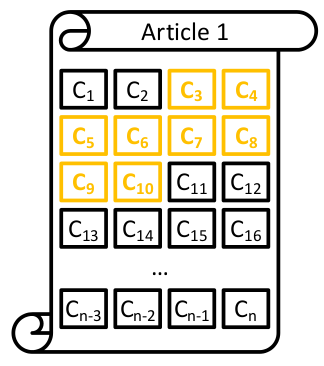
\includegraphics[scale=0.6]{bioqa/snippets.png}
\caption{An example of a golden snippet starting at offset 3 and ending at offset 10.}
\label{fig:snippets}
\end{figure}
\item F-measure:
\begin{align}
F = 2 \cdot \dfrac{P\cdot R}{P + R} \tag{Harmonic mean of Precision and Recall}
\end{align}
\item Average Precision (AP):
\begin{align}
AP &= \dfrac{\sum^{|L|}_{r=1} P(r) \cdot rel(r)}{L_R} \tag{see below}
\end{align} 
Where, for any given query $q_i$ and a golden set of items:
\begin{itemize}
\item $|L|$ is the total number of items.
\item $|L_R|$ is the number of relevant items. 
\item $P(r)$ is the precision for a list containing the first $r$ items.
\item $rel(r)$ is an indicator function for the existence of item $r$ in the golden set (i.e., it returns 1 if the $r$th item is relevant, and 0 otherwise).
\end{itemize}
\item Mean Average Precision (MAP):
\begin{align}
MAP &= \frac{1}{n} \sum^n_{i=1}AP_i  \tag{To get the average precision for list of queries $q_1, q_2, \dots, q_n$.}
\end{align}
\item Geometric Mean Average Precision (GMAP):
\begin{align}
GMAP &= \sqrt[n]{\prod^n_{i=1}(AP_i + \epsilon)} \tag{with some small $\epsilon$ for cases where $AP_i=0$}
\end{align}
GMAP is similar to MAP, only used to further penalize low performing queries.
\end{itemize}

\section{Archetype}
\subsection{Typesystem}
For this milestone, you are required to use the typesystem \verb|OAQATypes.xml| included in the archetype. Note however, you are only required to use the types defined in \ref{ref:mappings} and their supertype ancestry. You are of course welcome to extend the typesystem and/or use any other preexisting types. Most importantly. it is imperative that you use the inherited \verb|uri| and \verb|rank| attributes, as we will use them for evaluation.
\begin{figure}[h!]
\begin{longtable}{c|P{6cm}}
\textbf{BioASQ Type} & \textbf{UIMA Type}\\\hline
Result (supertype) &   \begin{itemize} \item \verb|edu.cmu.lti.oaqa.type.retrieval.SearchResult| \begin{itemize} \item \verb|uri| \item \verb|rank| \end{itemize} \end{itemize} \\\hline
Snippet & \begin{itemize} \item \verb|edu.cmu.lti.oaqa.type.retrieval.Passage| \begin{itemize} \item \verb|uri| (inherited) \item \verb|rank| (inherited) \end{itemize}  \end{itemize} \\\hline
\end{longtable}
\label{ref:mappings}
\caption{Typesystem Mapping}
\end{figure}
\subsection{Web Services}
\label{subsec:WebServices}
Unlike in M1, there is no client for M2. To access the web service below you will simply query \url{http://metal.lti.cs.cmu.edu:30002/pmc/PMID} with the PMID you retrieved from the previous services.
\begin{itemize}
\item Full Document Sources: a service for accessing the \emph{PMC} full text articles, with the same input parameters and output parameters as aforementioned, with the only difference being that the articles returned contain in addtion the full text.
\end{itemize}
\subsection{Data}
In the archetype you will also find \verb|BioASQ-SampleData1B.json| containing an annotated version of the 29 sample questions shown in M0. We also provide you with a convenience class \verb|JsonCollectionReaderHelper.java| to read from JSON format. 





\section{Creating Maven project from the archetype}

For this homework, we create another archetype called
\texttt{hellobioqa-archetype} to help you quickly get your development started.
We briefly show you the process you've gone through for your Homework 1.

\begin{enumerate}

\item Open your Eclipse's \textbf{Preferences} window, and navigate to
\textbf{Maven} $\rightarrow$ \textbf{Archetypes}, and click \textbf{Add Remote
Catalog\ldots}.

\item Type the following URL into the \textbf{Catalog File} field.

\small
\begin{verbatim}
http://ziy.github.com/hellobioqa-archetype/repository/archetype-catalog.xml
\end{verbatim}
\normalsize

Optionally, you can add a \textbf{Description} for this catalog, for example
``HelloBioQA Catalog''. Then click \textbf{OK} on the \textbf{Remote Archetype
Catalog} window and another \textbf{OK} on the \textbf{Preferences} window.

\item Include the following lines in your \texttt{settings.xml} in order to
download the artifact if you didn't do so in Homework 1.

\lstinputlisting[language=XML,float,linewidth=1.1\textwidth,caption=Configuring settings.xml,label=settings]{settings.xml}

\item Now you can follow almost the same steps to import to Eclipse as you did
for Homework 1. Since we have created the archetype for you, remember to
unselect \textbf{Create a simple project (skip archetype selction)}. Then click
\textbf{Next}.
 
\item Here you can select ``HelloBioQA Catalog'' (or other names you specified
in the previous step) or ``All Catalogs'' in the drop-down menu for
\textbf{Catalog}. Then, type in ``hellobioqa-archetype'' (without quotes) in the \textbf{Filter}
field, and in order to get the latest snapshot archetypes, you need to check
\textbf{Include snapshot archetypes} as well. Select the archetype listed below,
and click next to continue.

\item In the next window, you are asked to specify the \textbf{Group Id} and
\textbf{Artifact Id}. Similar to Homework 0 and 1, the Group Id is

\begin{center}
\textbf{edu.cmu.lti.11791.f13.hw2}
\end{center}

and Artifact Id is

\begin{center}
\textbf{hw2-teamXX}
\end{center}

with XX being your team number. Since we also included two sample components for
retrieval strategist and passage extraction within a particular, remember to
specify \texttt{Package} as

\begin{center}
\textbf{edu.cmu.lti.oaqa.openqa.hellobioqa}
\end{center}

See Figure \ref{fig:package-name}. Then click \textbf{Finish}.

\begin{figure}[t]
\centering
\includegraphics[scale=0.3]{package-name}
\caption{Parameters to create a Maven artifact from archetype\label{fig:package-name}}
\end{figure}

\item You need to edit the \texttt{pom.xml} file to type in the SCM information
of your GitHub repository for Homework 2 as you did in Homework 0.

\item You also need to manually edit the \texttt{launches/hellobioqa.launch}
file. Open the file, replace the \verb|${project_name}| with your project name
(e.g., \verb|hw2-team00|).

\item Probably you want to add another line into launch file to give extra
memory to run the pipeline, like the following

\begin{verbatim}
<stringAttribute key="org.eclipse.jdt.launching.VM_ARGUMENTS" value="-Xmx1g"/>
\end{verbatim}

\item Same as before, you probably need to right-click the project name, and
click \textbf{Maven} $\rightarrow$ \textbf{Update Project} to download the
dependencies.

\end{enumerate}

You can see that we have included

\begin{itemize}

\item the \texttt{pom.xml}. You can go to the \textbf{Dependencies} tab after
you double-click the pom file, and you will be able to see your project only
depends on \texttt{helloqa} project, which brings simple implementations for all
the phases described in \texttt{baseqa} project. You won't need any direct
dependency on any UIMA SDK package, which are essential to your Homework 1.

If you want to take a look at what are inside \texttt{helloqa} project and
other indirect dependencies, you can unfold the \texttt{Maven Dependencies}
folder under your project name in the Package Explorer View.

\item input file in the \texttt{src/main/resources/input} folder, and
gold-standard annotations in the \texttt{src/main/resources/gs} folder. If you
are interested in their contents, you can open them with a text editor.

\item several descriptors under \texttt{src/main/resources/hellobioqa} directory
and subdirectories. All of them are specific to the hellobioqa task, and
actually, you can find more descriptors from dependencies, e.g.,
\texttt{helloqa}, \texttt{jdbc-provider}, etc. These descriptors can also be
considered to incorporate in your project.

\item the main yaml \texttt{src/main/resources/hellobioqa/hellobioqa.yaml}

\item an Eclipse launch file \texttt{launches/hellobioqa.launch}. To run the
pipeline, you can right-click this file in the Package Explorer View, and then
click \textbf{Run As} $\rightarrow$ \textbf{hellobioqa}.

\item a local database version of the cse repository
\texttt{data/oaqa-eval.db3}. All your experiment intermediate result and
evaluation results will be permanently stored here (unless you manually delete
table entries), and you will find the file may grow to several megabytes after
thundreds of experiments. Therefore, we suggest you should not commit this file
to the GitHub repository, instead you can \texttt{git ignore} this file to avoid
this huge file bothering you every time you commit your project.

\end{itemize}

Before you commit and push all the initial code changes to GitHub repository, we
suggest you to first test if you can successfully run the pipeline.

\begin{enumerate}

\item Right-click this file in the Package Explorer View, and then click
\textbf{Run As} $\rightarrow$ \textbf{hellobioqa}. Wait until all 28 questions
are processed, and the evaluation results are printed to the console, and you
find no exceptions are thrown.

\item Git-ignore \texttt{data/oaqa-eval.db3}\footnote{Since your team member
also needs the database file to run experiment, the team leader can add it to
the index first then remove it after team members clone the project to their
machines, or all the members can download an empty file from here:
\url{https://github.com/oaqa/helloqa/blob/a051e1233be92bca309ff8761835fce412f6bfd5/data/oaqa-eval.db3?raw=true},
and put it under \texttt{data/}.}, and commit/push all other code changes to the
GitHub repository. Remember to commit the .project file, .classpath file and all
other important configuration files from your project root directory, and it
will be helpful for your team members to directly import an existing project.

\item Now, other team members are able to clone the repository to their
workspaces and start working on particular task. When you are asked to
\textbf{Select a wizard to use for importing projects}, don't forget to select
\textbf{Import existing projects} as long as your team leader commited .project
and .classth to the repository.

\end{enumerate}

